\subsection{Conceptual introduction}
\begin{frame}
\frametitle{sets}
\begin{center}	
			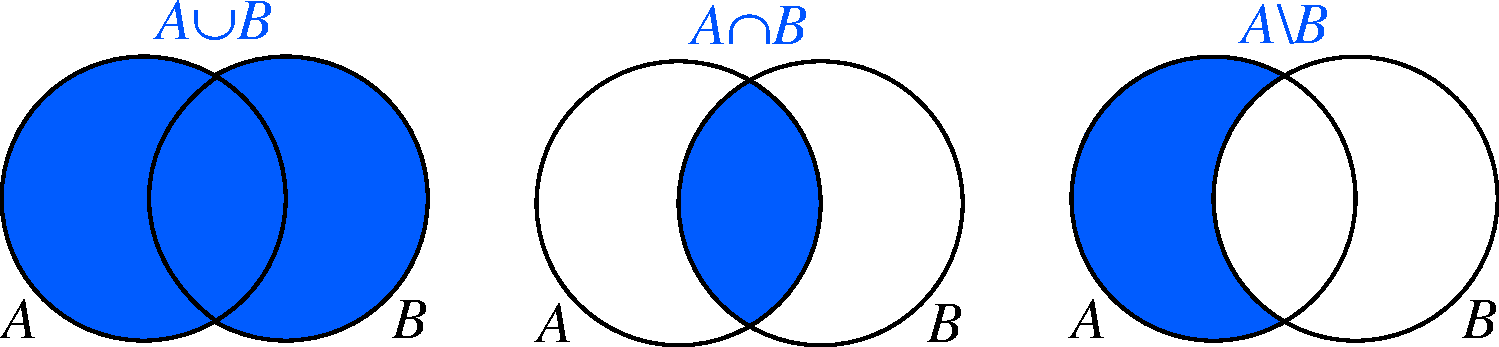
\includegraphics[scale=0.45]{fig/setth.pdf}
	\end{center}		
\end{frame}

\begin{frame}
\frametitle{probability measure}
\begin{center}	
			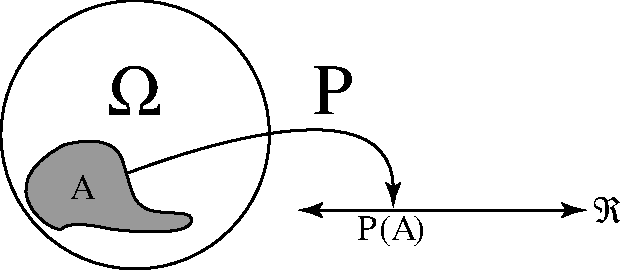
\includegraphics[scale=0.45]{fig/propmeas5.pdf}
	\end{center}		
\end{frame}

\begin{frame}
\frametitle{probability axioms}
\begin{center}	
			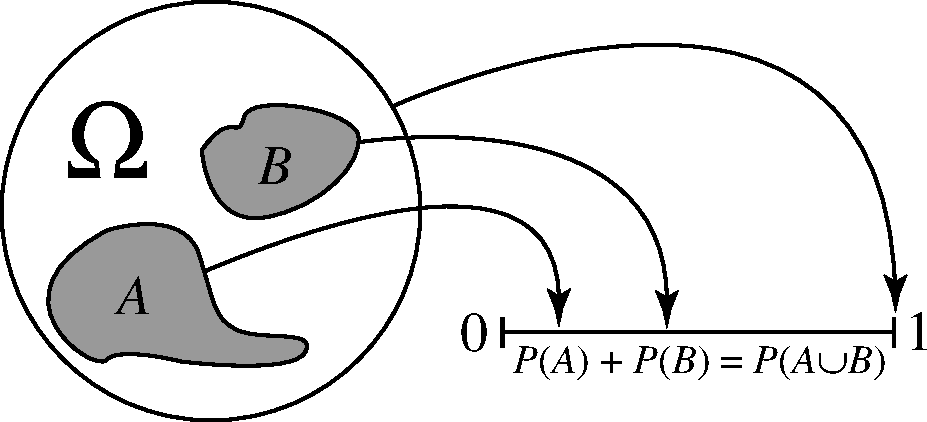
\includegraphics[scale=0.45]{fig/probthax7.pdf}
	\end{center}		
\end{frame}

\begin{frame}
\frametitle{conditional probability}
\begin{center}	
			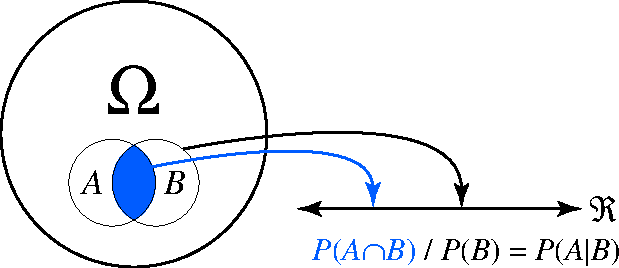
\includegraphics[scale=0.45]{fig/condprob10.pdf}
	\end{center}		
\end{frame}

\begin{frame}
\frametitle{random variables}
\begin{center}	
			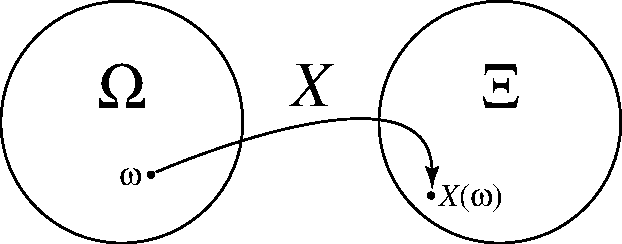
\includegraphics[scale=0.45]{fig/randvar15.pdf}
	\end{center}		
\end{frame}

\begin{frame}
\frametitle{probability densities}
\begin{center}	
			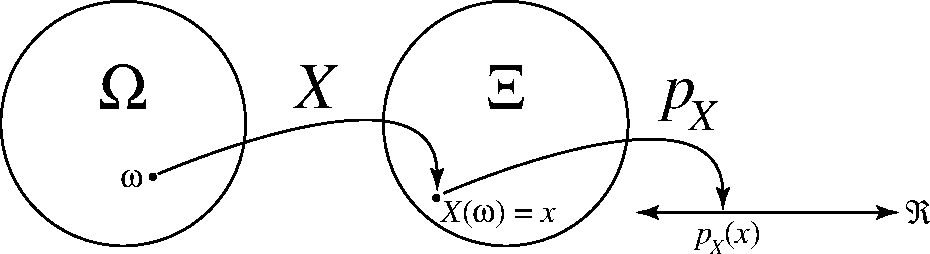
\includegraphics[scale=0.45]{fig/probdensity17.pdf}
	\end{center}		
\end{frame}

\begin{frame}
\frametitle{joint probability densities}
\begin{center}	
			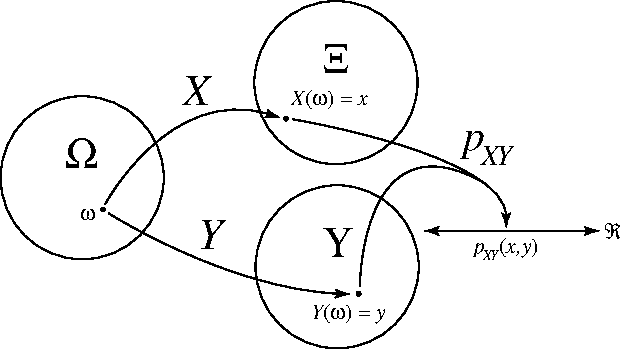
\includegraphics[scale=0.45]{fig/probjointdens18.pdf}
	\end{center}		
\end{frame}

\begin{frame}
\frametitle{the reality}
\begin{center}	
			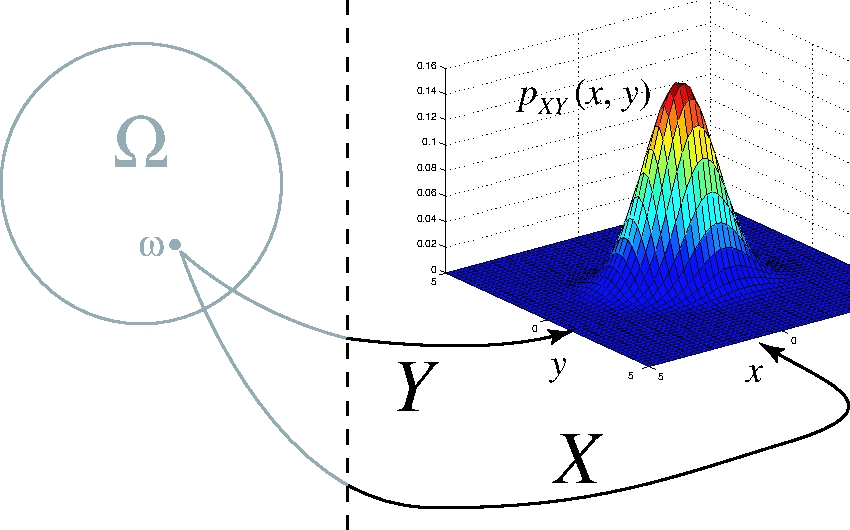
\includegraphics[scale=0.45]{fig/probreality19.pdf}
	\end{center}		
\end{frame}

\subsection{Measure theory}
\begin{frame}
\begin{itemize}
\item For the general theory of measure spaces, we first need a \emph{measurable space} $(\Omega, \Sigma)$, that is a set equipped with a collection $\Sigma$ of \textbf{measurable sets} complete under certain operations. Then this becomes a measure space $(\Omega, \Sigma, \mu)$ by throwing in a function $\mu$ from $\Sigma$ to a space of values (such as the real line) that gets along with the set-theoretic operations that $\Sigma$ has. If $E$ is a measurable set, then $\mu(E)$ is called the \textbf{measure} of $E$ with respect to $\mu$. \cite{Insua2012, NLab}
\end{itemize}
\end{frame}

\begin{frame}
\begin{enumerate}
\item Given a set $\Omega$, 
\item a \textbf{$\sigma$-algebra} is a collection of subsets of $\Omega$ that is closed under complementation, countable unions, and countable intersections. 
\item A \textbf{measurable space}, by the usual modern definition, is a set $\Omega$ equipped with a $\sigma$-algebra $\Sigma$. 
\item The elements of $\Sigma$ are called the \textbf{measurable sets} of $\Omega$ (or more properly, the measurable subsets of $(\Omega,\Sigma)$).
\end{enumerate}
\end{frame}

\begin{frame}
A \textbf{measure space} is a \textbf{measurable space} equipped with a \textbf{measure}. There are many different types of measures parametrized by the type of their codomains. Let $(\Omega, \Sigma)$ be a measurable space. A \textbf{probability measure} on $\Omega$ (due to Kolmogorov) is a function $\mu$ from the collection $\Sigma$ of measurable sets to the unit interval $[0,1]$ such that:

\begin{enumerate}%
\item The measure of the empty set is zero: $\mu(\emptyset) = 0$;
\item The measure of the entire space is one: $\mu(\Omega) = 1$;
\item Countable additivity: $\mu(\bigcup_{i = 1}^{\infty} S_i) = \sum_{i=1}^{\infty} \mu(S_i)$ whenever the $S_i$ are mutually disjoint sets|disjoint.
(Part of the latter condition is the requirement that the sum on the right-hand side must converge.)
\end{enumerate}
\end{frame}

\begin{frame}
It is sometimes stated (but in fact follows from the previous) that:

\begin{itemize}%
\item Finitary additivity: $\mu(S \cup T) = \mu(S) + \mu(T)$ whenever $S$ and $T$ are disjoint.
\item $\mu$ is increasing: $\mu(A) \leq \mu(B)$ if $A \subseteq B$.

\end{itemize}
\end{frame}

\begin{frame}
Measures can be thought of in terms of integrals and densities are defined in terms of measures. Let $A$ be, for example, one of the measurable sets from the collection of measurable sets, $\Sigma$, of our sample space $\Omega$.

\begin{itemize}
\item $\mu(A) = \int_A dx$ or $\mu(A) = \int_A p(x)dx$
\item $\mu(A)$ represents the mass of A which can be interpreted geometrically as an \emph{abstract volume} or probabilistically as \emph{the probability mass of the event "random variable X takes a value within A"}
\item A \textbf{density} can then be defined intuitively as a function that transforms some measure $\mu_1$ into a measure $\mu_2$ by pointwise reweighting on the sample space $\Omega$. Thus, densities are always relative measures.
\item $d \mu_2 (x) = f(x) d \mu_1 (x)$ or $\frac{d \mu_2}{d \mu_2} (x) = f(x)$
\end{itemize}

\end{frame}

\begin{frame}
Does a density always exist?

\begin{itemize}
\item A density function $f$ is thus a function that is integrated to obtain information in terms of measure $\mu_2$ from information in terms of measure $\mu_1$. 
\item $\mu_2 (A) = \int_A d \mu_2 (x) = \int_A f(x) d \mu_1 (x)$ is not defined if $\mu_1(A) = 0$ and $\mu_2(A) \neq 0$.
\item If this is never the case for all $A \in \Sigma$, then $\mu_2$ is referred to as \emph{absolutely continuous} with respect to $\mu_1$ and this relationship is written $\mu_2 \ll \mu_1$.
\item This conclusion is formalized in the \textbf{Radon-Nikodym theorem} which states that $\mu_2$ has a density with respect to $\mu_1$ if and only if $\mu_2 \ll \mu_1$.
\end{itemize}
$\ldots$ so the answer is $\ldots$ no, which is the reason for going through all this abstract stuff
\end{frame}